\documentclass[11pt,a4paper]{report}
\usepackage[textwidth=37em,vmargin=30mm]{geometry}
\usepackage{calc,xunicode,amsmath,amssymb,paralist,enumitem,tabu,booktabs,datetime2,xeCJK,xeCJKfntef,listings}
\usepackage{tocloft,fancyhdr,tcolorbox,xcolor,graphicx,eso-pic,xltxtra,xelatexemoji}

\newcommand{\envyear}[0]{2024}
\newcommand{\envdatestr}[0]{2024-11-11}
\newcommand{\envfinaldir}[0]{webdb/2024/20241111/final}

\usepackage[hidelinks]{hyperref}
\hypersetup{
    colorlinks=false,
    pdfpagemode=FullScreen,
    pdftitle={Web Digest - \envdatestr}
}

\setlength{\cftbeforechapskip}{10pt}
\renewcommand{\cftchapfont}{\rmfamily\bfseries\large\raggedright}
\setlength{\cftbeforesecskip}{2pt}
\renewcommand{\cftsecfont}{\sffamily\small\raggedright}

\setdefaultleftmargin{2em}{2em}{1em}{1em}{1em}{1em}

\usepackage{xeCJK,xeCJKfntef}
\xeCJKsetup{PunctStyle=plain,RubberPunctSkip=false,CJKglue=\strut\hskip 0pt plus 0.1em minus 0.05em,CJKecglue=\strut\hskip 0.22em plus 0.2em}
\XeTeXlinebreaklocale "zh"
\XeTeXlinebreakskip = 0pt


\setmainfont{Brygada 1918}
\setromanfont{Brygada 1918}
\setsansfont{IBM Plex Sans}
\setmonofont{JetBrains Mono NL}
\setCJKmainfont{Noto Serif CJK SC}
\setCJKromanfont{Noto Serif CJK SC}
\setCJKsansfont{Noto Sans CJK SC}
\setCJKmonofont{Noto Sans CJK SC}

\setlength{\parindent}{0pt}
\setlength{\parskip}{8pt}
\linespread{1.15}

\lstset{
	basicstyle=\ttfamily\footnotesize,
	numbersep=5pt,
	backgroundcolor=\color{black!5},
	showspaces=false,
	showstringspaces=false,
	showtabs=false,
	tabsize=2,
	captionpos=b,
	breaklines=true,
	breakatwhitespace=true,
	breakautoindent=true,
	linewidth=\textwidth
}






\newcommand{\coverpic}[2]{
    % argv: itemurl, authorname
    Cover photo by #2~~(\href{#1}{#1})
}
\newcommand{\makeheader}[0]{
    \begin{titlepage}
        % \newgeometry{hmargin=15mm,tmargin=21mm,bmargin=12mm}
        \begin{center}
            
            \rmfamily\scshape
            \fontspec{BaskervilleF}
            \fontspec{Old Standard}
            \fontsize{59pt}{70pt}\selectfont
            WEB\hfill DIGEST
            
            \vfill
            % \vskip 30pt
            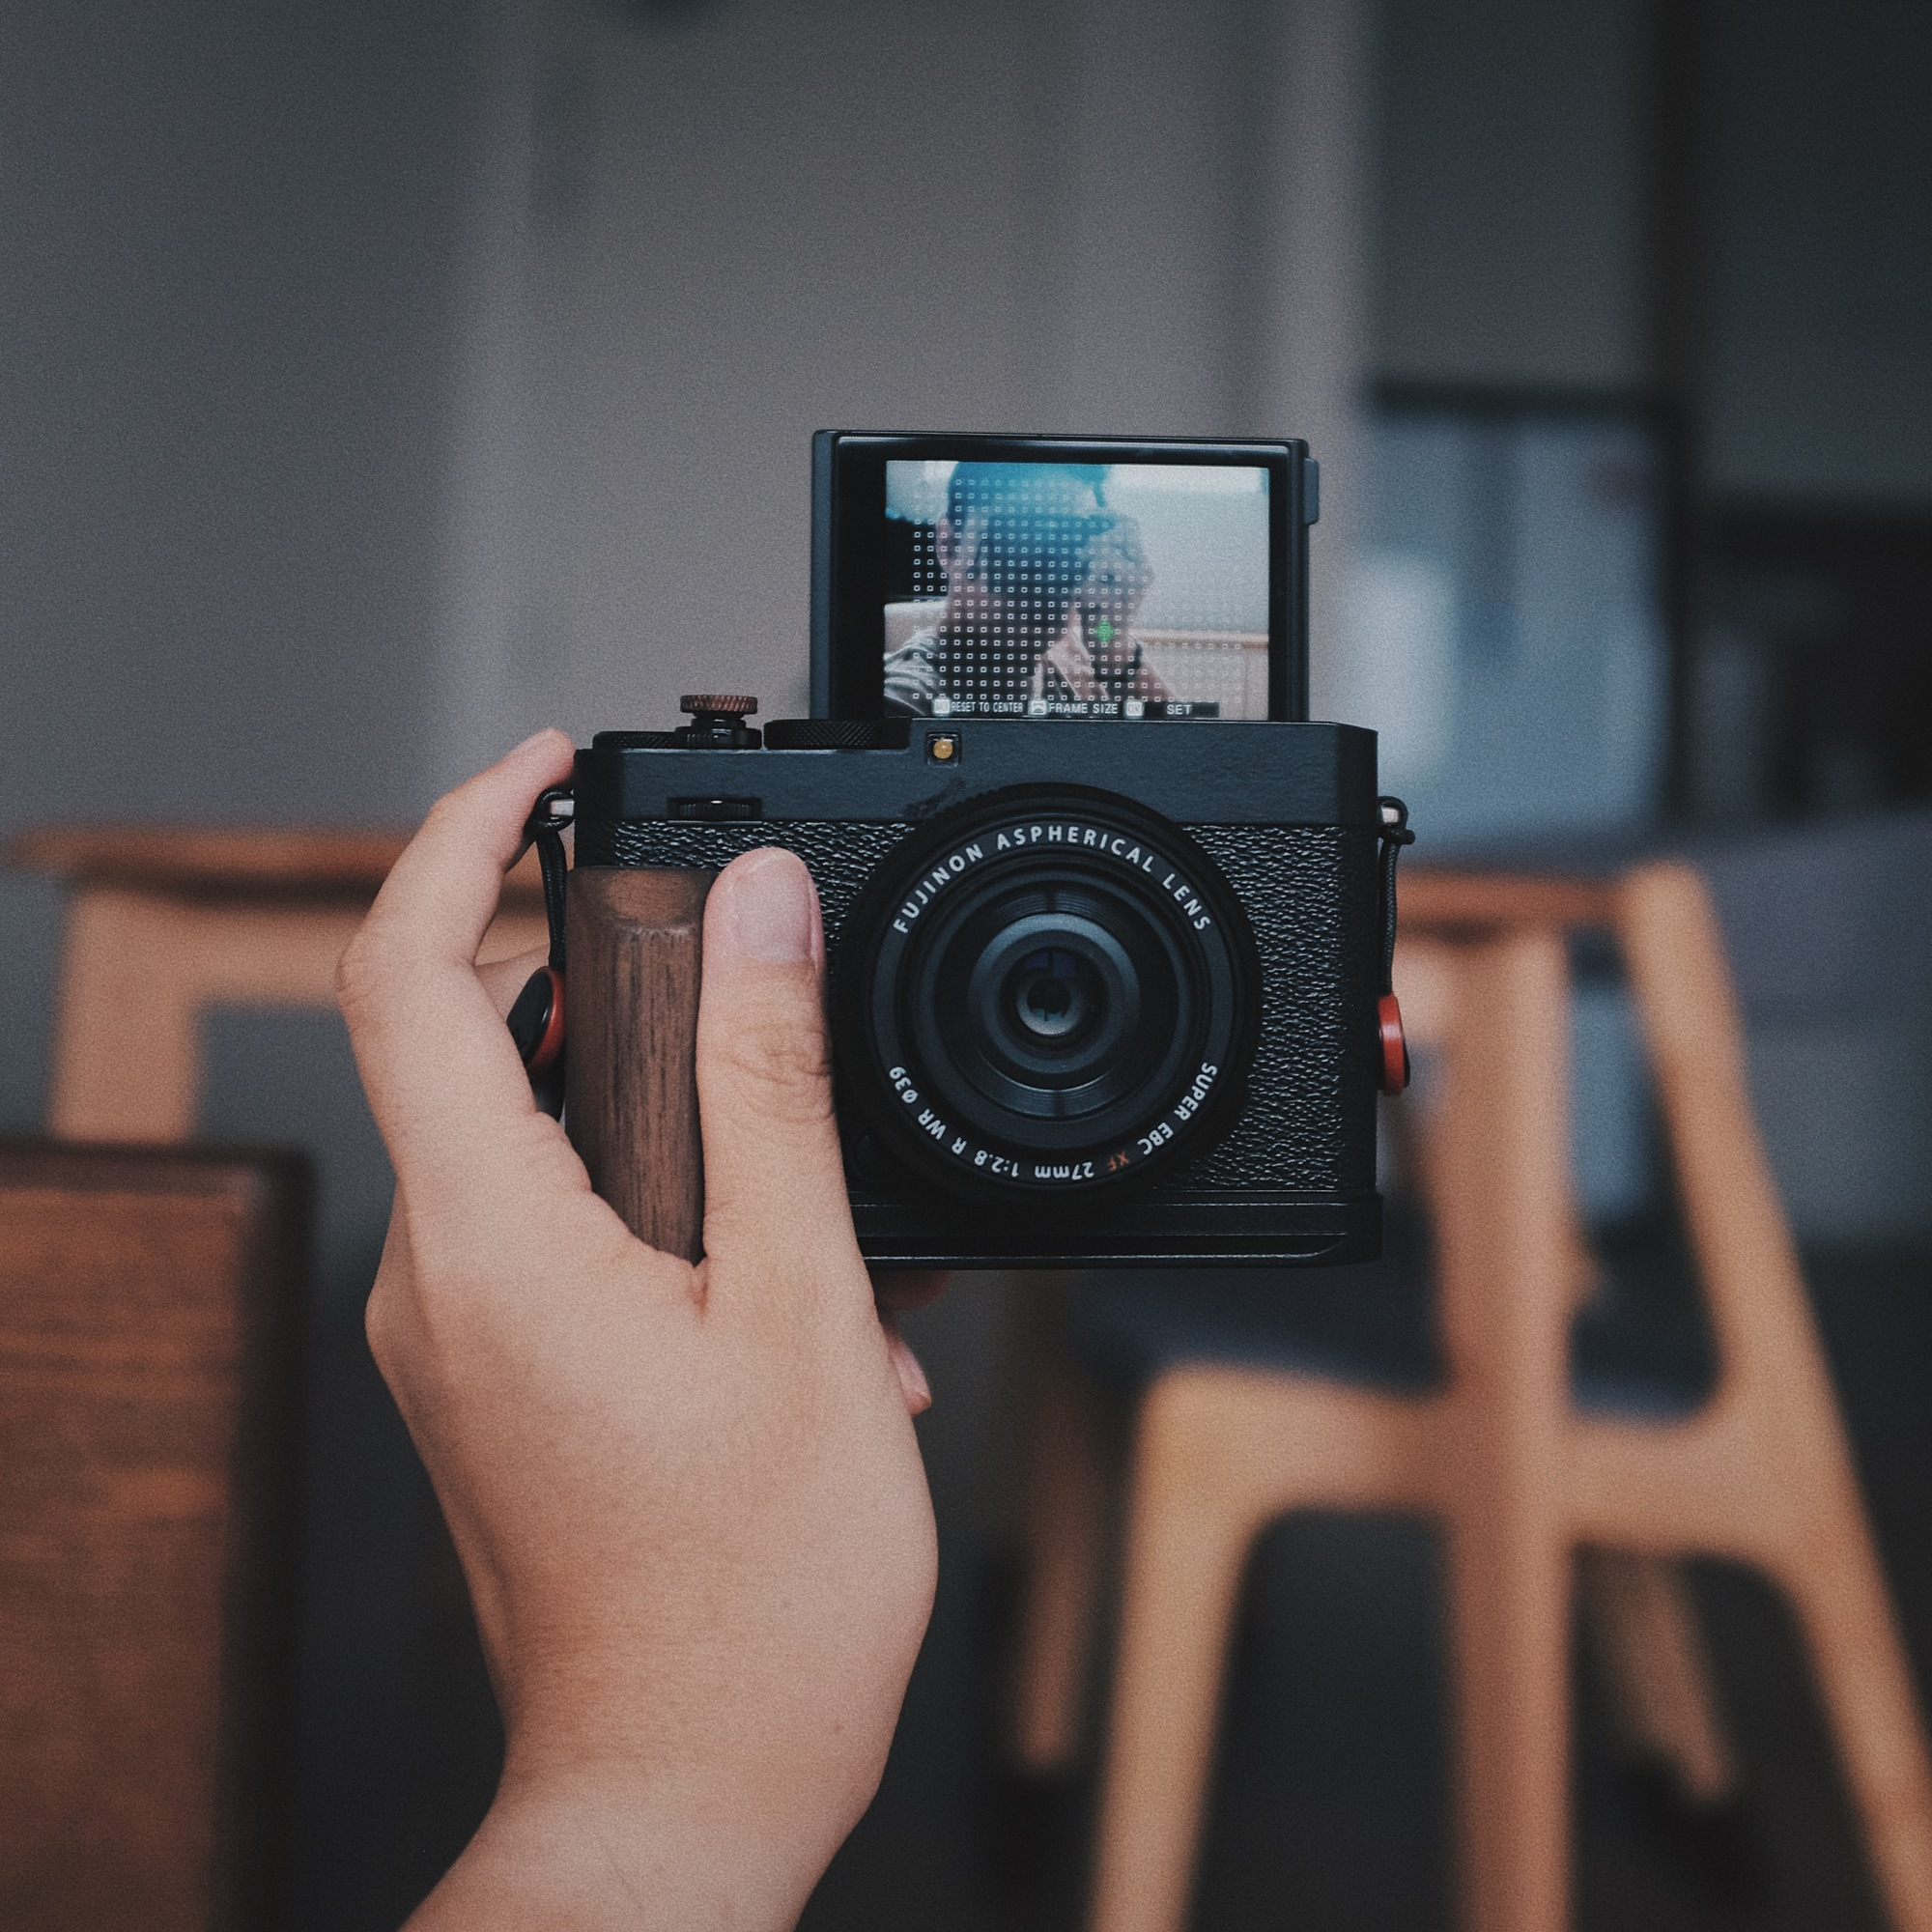
\includegraphics[width=\linewidth]{\envfinaldir/coverpic-prod.jpg}\par
            % \vskip 30pt
            \vfill

            \normalsize\rmfamily\scshape
            \copyright{} The Web Digest Project \hfill\large \envdatestr
        \end{center}
    \end{titlepage}
    % \restoregeometry
}
\newcommand{\simplehref}[1]{%
    \textcolor{blue!80!green}{\href{#1}{#1}}%
}
\renewcommand{\contentsname}{\center\Huge\sffamily\bfseries Contents\par\vskip 20pt}
\newcounter{ipartcounter}
\setcounter{ipartcounter}{0}
\newcommand{\ipart}[1]{
    % \vskip 20pt
    \clearpage
    \stepcounter{ipartcounter}
    \phantomsection
    \addcontentsline{toc}{chapter}{#1}
    % \begin{center}
    %     \Huge
    %     \sffamily\bfseries
    %     #1
    % \end{center}
    % \vskip 20pt plus 7pt
}
\newcounter{ichaptercounter}
\setcounter{ichaptercounter}{0}
\newcommand{\ichapter}[1]{
    % \vskip 20pt
    \clearpage
    \stepcounter{ichaptercounter}
    \phantomsection
    \addcontentsline{toc}{section}{\numberline{\arabic{ichaptercounter}}#1}
    \begin{center}
        \Huge
        \sffamily\bfseries
        #1
    \end{center}
    \vskip 20pt plus 7pt
}
\newcommand{\entrytitlefont}[1]{\subsection*{\raggedright\Large\sffamily\bfseries#1}}
\newcommand{\entryitemGeneric}[2]{
    % argv: title, url
    \parbox{\linewidth}{
        \entrytitlefont{#1}\par\vskip 5pt
        \footnotesize\ttfamily\mdseries
        \simplehref{#2}
    }\vskip 11pt plus 11pt minus 1pt
}
\newcommand{\entryitemGithub}[3]{
    % argv: title, url, desc
    \parbox{\linewidth}{
        \entrytitlefont{#1}\par\vskip 5pt
        \footnotesize\ttfamily\mdseries
        \simplehref{#2}\par\vskip 5pt
        \small\rmfamily\mdseries#3
    }\vskip 11pt plus 11pt minus 1pt
}
\newcommand{\entryitemAp}[3]{
    % argv: title, url, desc
    \parbox{\linewidth}{
        \entrytitlefont{#1}\par\vskip 5pt
        \footnotesize\ttfamily\mdseries
        \simplehref{#2}\par\vskip 5pt
        \small\rmfamily\mdseries#3
    }\vskip 11pt plus 11pt minus 1pt
}
\newcommand{\entryitemHackernews}[3]{
    % argv: title, hnurl, rawurl
    % \parbox{\linewidth}{
    %     \entrytitlefont{#1}\par\vskip 5pt
    %     \footnotesize\ttfamily\mdseries
    %     \simplehref{#3}\par
    %     \textcolor{black!50}{\href{#2}{#2}}
    % }\vskip 11pt plus 11pt minus 1pt
    \begin{minipage}{\linewidth}
            \entrytitlefont{#1}\par\vskip 5pt
            \footnotesize\ttfamily\mdseries
            \simplehref{#3}\par
            \textcolor{black!50}{\href{#2}{#2}}
    \end{minipage}\par\vskip 11pt plus 11pt minus 1pt
}







\begin{document}

\makeheader

\tableofcontents\clearpage




\ipart{Developers}
\ichapter{Hacker News}
\entryitemTwoLinks{Procrastination and the fear of not being good enough}{https://news.ycombinator.com/item?id=42101327}{https://swapnilchauhan.com/blog/procrastination-and-the-fear-of-not-being-good-enough}

\entryitemTwoLinks{Salary expectations questions – How should you answer them? (2020)}{https://news.ycombinator.com/item?id=42101107}{https://fearlesssalarynegotiation.com/salary-expectations-interview-question/}

\entryitemTwoLinks{Physical Intelligence's first generalist policy AI can finally do your laundry}{https://news.ycombinator.com/item?id=42098236}{https://www.physicalintelligence.company/blog/pi0}

\entryitemTwoLinks{LLMs have reached a point of diminishing returns}{https://news.ycombinator.com/item?id=42097774}{https://garymarcus.substack.com/p/confirmed-llms-have-indeed-reached}

\entryitemTwoLinks{Grim Fandango}{https://news.ycombinator.com/item?id=42097261}{https://www.filfre.net/2024/11/grim-fandango/}

\entryitemTwoLinks{Show HN: Jaws – a JavaScript to WASM ahead-of-time compiler}{https://news.ycombinator.com/item?id=42095879}{https://github.com/drogus/jaws}

\entryitemTwoLinks{IronCalc – Open-Source Spreadsheet Engine}{https://news.ycombinator.com/item?id=42095292}{https://www.ironcalc.com/}

\entryitemTwoLinks{Scientist treated her own cancer with viruses she grew in the lab}{https://news.ycombinator.com/item?id=42094573}{https://www.nature.com/articles/d41586-024-03647-0}

\entryitemTwoLinks{Memories are not only in the brain, human cell study finds}{https://news.ycombinator.com/item?id=42094427}{https://medicalxpress.com/news/2024-11-memories-brain-human-cell.html}

\entryitemTwoLinks{NASA remains silent on why crew went to hospital after dragon splashdown}{https://news.ycombinator.com/item?id=42092385}{https://gizmodo.com/nasa-remains-stubbornly-silent-on-dragon-splashdown-that-sent-crew-to-hospital-2000522187}

\entryitemTwoLinks{It's legal for police to use deception in interrogations. Some want that to end}{https://news.ycombinator.com/item?id=42091423}{https://text.npr.org/nx-s1-4974964}

\entryitemTwoLinks{Claude AI to process secret government data through new Palantir deal}{https://news.ycombinator.com/item?id=42091043}{https://arstechnica.com/ai/2024/11/safe-ai-champ-anthropic-teams-up-with-defense-giant-palantir-in-new-deal/}

\entryitemTwoLinks{What Is a Staff Engineer?}{https://news.ycombinator.com/item?id=42090771}{https://nishtahir.com/what-is-a-staff-engineer/}

\entryitemTwoLinks{Notes on Guyana}{https://news.ycombinator.com/item?id=42090704}{https://mattlakeman.org/2024/11/08/notes-on-guyana/}

\entryitemTwoLinks{I quit Google to work for myself (2018)}{https://news.ycombinator.com/item?id=42090430}{https://mtlynch.io/why-i-quit-google/}

\entryitemTwoLinks{Mitochondria Are Alive}{https://news.ycombinator.com/item?id=42088758}{https://www.asimov.press/p/mitochondria}

\entryitemTwoLinks{The Weeds Are Winning}{https://news.ycombinator.com/item?id=42087770}{https://www.technologyreview.com/2024/10/10/1105034/weeds-climate-change-genetic-engineering-superweeds-food/}

\entryitemTwoLinks{How to Fix the Electoral College}{https://news.ycombinator.com/item?id=42087694}{https://www.federicolopriore.com/en/posts/electoral-college/}

\entryitemTwoLinks{Perceptually lossless (talking head) video compression at 22kbit/s}{https://news.ycombinator.com/item?id=42084977}{https://mlumiste.com/technical/liveportrait-compression/}

\entryitemTwoLinks{Principles for product velocity}{https://news.ycombinator.com/item?id=42084753}{https://ssoready.com/blog/from-the-founders/methodology-is-bullshit/}\ichapter{Phoronix}
\entryitemGeneric{\hskip 0pt{}Linux 6.12-rc7 Released: Linux 6.12 Stable On Track For Release Next Sunday}{https://www.phoronix.com/news/Linux-6.12-rc7-Released}

\entryitemGeneric{\hskip 0pt{}Arch Linux Powered CachyOS Pulls In THP Shrinker \& AMD Cache Optimizer}{https://www.phoronix.com/news/CachyOS-November-2024}

\entryitemGeneric{\hskip 0pt{}Linux Optimization Patches Significantly Speed-Up Debuggers Using /proc/kcore}{https://www.phoronix.com/news/Linux-Faster-Dragn-proc-kcore}

\entryitemGeneric{\hskip 0pt{}Debcow Optimizing Debian Packages For Copy-On-Write File-Systems}{https://www.phoronix.com/news/Debcow-Debian-DEBs-CoW-FS}

\entryitemGeneric{\hskip 0pt{}Linux Support For Apple's Latest Magic Trackpad USB-C Model}{https://www.phoronix.com/news/Linux-2024-Apple-Magic-Trackpad}

\entryitemGeneric{\hskip 0pt{}Wine-Staging 9.21 Fixes Some Old Game Crashes \& Hangs Due To DirectMusic}{https://www.phoronix.com/news/Wine-Staging-9.21}

\entryitemGeneric{\hskip 0pt{}Niri 0.1.10 Scrollable-Tiling Wayland Compositor Brings Many Improvements}{https://www.phoronix.com/news/Niri-0.1.10-Wayland-Released}

\entryitemGeneric{\hskip 0pt{}Debian 12.8 Released With Many Bug Fixes \& Security Updates}{https://www.phoronix.com/news/Debian-12.8-Released}

\entryitemGeneric{\hskip 0pt{}Hyprland 0.45 Compositor Smooths Round Edges, Window Snapping For Floating Windows}{https://www.phoronix.com/news/Hyprland-0.45-Wayland}


\ipart{Developers~~~~(zh-Hans)}
\ichapter{Solidot}
\entryitemGeneric{\hskip 0pt{}过去四年私人飞机二氧化碳排放量大幅增长}{https://www.solidot.org/story?sid=79732}

\entryitemGeneric{\hskip 0pt{}Firefox 以及 Thunderbird 1.0 发布二十周年}{https://www.solidot.org/story?sid=79731}

\entryitemGeneric{\hskip 0pt{}Fedora KDE 将与 Fedora GNOME 处于同等位置}{https://www.solidot.org/story?sid=79730}

\entryitemGeneric{\hskip 0pt{}43 只猴子逃离南卡罗来纳实验室}{https://www.solidot.org/story?sid=79729}

\entryitemGeneric{\hskip 0pt{}海盗湾上没有海盗湾电视剧}{https://www.solidot.org/story?sid=79728}

\entryitemGeneric{\hskip 0pt{}三名角膜受损患者接受干细胞治疗后恢复视力}{https://www.solidot.org/story?sid=79727}

\entryitemGeneric{\hskip 0pt{}台积电将停止为大陆客户制造 7 纳米 AI 芯片}{https://www.solidot.org/story?sid=79726}

\entryitemGeneric{\hskip 0pt{}为什么湿狗想要抖掉身上的水?}{https://www.solidot.org/story?sid=79725}

\entryitemGeneric{\hskip 0pt{}张忠谋曾邀请黄仁勋担任台积电 CEO}{https://www.solidot.org/story?sid=79724}

\entryitemGeneric{\hskip 0pt{}为什么人脑与众不同}{https://www.solidot.org/story?sid=79723}

\entryitemGeneric{\hskip 0pt{}QNX 对非商业使用免费}{https://www.solidot.org/story?sid=79722}

\entryitemGeneric{\hskip 0pt{}中国人口连续两年负增长}{https://www.solidot.org/story?sid=79721}

\entryitemGeneric{\hskip 0pt{}中国专利申请量继续高居第一}{https://www.solidot.org/story?sid=79720}

\entryitemGeneric{\hskip 0pt{}每天运动五分钟有助于降低血压}{https://www.solidot.org/story?sid=79719}

\entryitemGeneric{\hskip 0pt{}祝融号发现火星古代海洋新证据}{https://www.solidot.org/story?sid=79718}

\entryitemGeneric{\hskip 0pt{}加拿大加密货币公司 CEO 被绑架和勒索 100 万美元}{https://www.solidot.org/story?sid=79717}

\entryitemGeneric{\hskip 0pt{}英特尔 Linux 补丁将旧版本的微码视为漏洞}{https://www.solidot.org/story?sid=79716}

\entryitemGeneric{\hskip 0pt{}亚马逊正在制作《质量效应》电视剧}{https://www.solidot.org/story?sid=79715}

\entryitemGeneric{\hskip 0pt{}俄罗斯屏蔽 Cloudflare 的 ECH 连接}{https://www.solidot.org/story?sid=79714}

\entryitemGeneric{\hskip 0pt{}COVID-19 干预措施改变了流感传播}{https://www.solidot.org/story?sid=79713}\ichapter{V2EX}
\entryitemGeneric{\hskip 0pt{}[iCloud] icloud 国区 2T 拼车}{https://www.v2ex.com/t/1088328}

\entryitemGeneric{\hskip 0pt{}[Apple] mac mini 都装些啥,求教?}{https://www.v2ex.com/t/1088327}

\entryitemGeneric{\hskip 0pt{}[Bitcoin] V2 站居然在 2011 年既然就可以用 btc 来答谢了,有人收到过吗?}{https://www.v2ex.com/t/1088326}

\entryitemGeneric{\hskip 0pt{}[VPS] x-ui 面板这样设置节点安全吗? vless+tls。flow 是 xtls-rprx-vision}{https://www.v2ex.com/t/1088325}

\entryitemGeneric{\hskip 0pt{}[问与答] 国行 POE 交换机能在北美用吗?}{https://www.v2ex.com/t/1088323}

\entryitemGeneric{\hskip 0pt{}[Apple] M4 Pro 初体验 代码/音响}{https://www.v2ex.com/t/1088322}

\entryitemGeneric{\hskip 0pt{}[装修] 燃气热水器怎么选?}{https://www.v2ex.com/t/1088321}

\entryitemGeneric{\hskip 0pt{}[问与答] 麦克风拾音问题,电脑麦克风重复拾取喇叭声音,但演唱会 KTV 不会?}{https://www.v2ex.com/t/1088320}

\entryitemGeneric{\hskip 0pt{}[程序员] 请教大佬们一个 chrome 侧边栏插件的开发问题,已经卡好几天了,问了 ai 也没解决}{https://www.v2ex.com/t/1088318}

\entryitemGeneric{\hskip 0pt{}[分享发现] 再现经典 Plinko}{https://www.v2ex.com/t/1088316}

\entryitemGeneric{\hskip 0pt{}[分享发现] 某小城市,京东快递员要求上门必须本人当面签收+端着包裹拍照,不允许放家门口。京东客服表示也只能这样}{https://www.v2ex.com/t/1088315}

\entryitemGeneric{\hskip 0pt{}[macOS] 关于 macOS 在内网使用 finder 通过 http://192.168.xxx.xx 连接 nas(即 finder 自带的连接服务器)后报错 100004}{https://www.v2ex.com/t/1088314}

\entryitemGeneric{\hskip 0pt{}[PayPal] 底特律居民明年将能够使用 PayPal 以加密货币缴纳税款。}{https://www.v2ex.com/t/1088313}

\entryitemGeneric{\hskip 0pt{}[macOS] 我的 MacBook 电脑总在运行一段时间之后, Command+Q 失效}{https://www.v2ex.com/t/1088312}

\entryitemGeneric{\hskip 0pt{}[Android] 小米手机无法通过 hostname 访问局域网设备}{https://www.v2ex.com/t/1088311}

\entryitemGeneric{\hskip 0pt{}[问与答] Java 论坛源码求推荐}{https://www.v2ex.com/t/1088310}

\entryitemGeneric{\hskip 0pt{}[分享发现] 我可能要远离 chrome 了}{https://www.v2ex.com/t/1088309}

\entryitemGeneric{\hskip 0pt{}[咖啡] 瑞幸 app 一天访问了我的位置信息 604 次,而我只是点了一杯咖啡而已}{https://www.v2ex.com/t/1088308}

\entryitemGeneric{\hskip 0pt{}[分享发现] 独立开发一个月,收入竟然逼近}{https://www.v2ex.com/t/1088307}

\entryitemGeneric{\hskip 0pt{}[问与答] 老二出生了,求起名字}{https://www.v2ex.com/t/1088306}

\entryitemGeneric{\hskip 0pt{}[分享发现] pdd 支持上海国补了}{https://www.v2ex.com/t/1088305}

\entryitemGeneric{\hskip 0pt{}[Apple] 老外设计的 Mac mini M4 开机键,优雅多了。}{https://www.v2ex.com/t/1088304}

\entryitemGeneric{\hskip 0pt{}[问与答] 求教,在腾讯云上用 docker 部署 dreamacro/clash 会被封禁吗}{https://www.v2ex.com/t/1088303}

\entryitemGeneric{\hskip 0pt{}[问与答] 讲一下今年接的私活,没拿到钱,说说感想~}{https://www.v2ex.com/t/1088302}

\entryitemGeneric{\hskip 0pt{}[Apple] Apple TV 上是否有类似 IINA、Movist Pro、nPlayer 的纯粹播放器}{https://www.v2ex.com/t/1088301}

\entryitemGeneric{\hskip 0pt{}[iPhone] 港版 iPhone16 支持 FaceTime Audio 音频通话,在大陆怎么使用呢?}{https://www.v2ex.com/t/1088300}

\entryitemGeneric{\hskip 0pt{}[Apple] 求教一套妙控键鼠如何在 2 台 Mac 间切换}{https://www.v2ex.com/t/1088298}

\entryitemGeneric{\hskip 0pt{}[NAS] DIY NAS (All in boom) 回来交作业了}{https://www.v2ex.com/t/1088297}

\entryitemGeneric{\hskip 0pt{}[求职] 12 年全栈开发( Java /C\#/iOS/Android/Vue/React),找远程工作,或者承接外包项目。}{https://www.v2ex.com/t/1088296}

\entryitemGeneric{\hskip 0pt{}[程序员] 基于 MediaPipe 和 HaGRID 数据集做了个手势分类}{https://www.v2ex.com/t/1088295}

\entryitemGeneric{\hskip 0pt{}[区块链] BTC 迫近 80k USD, V 站对此的讨论好像几乎没有}{https://www.v2ex.com/t/1088294}

\entryitemGeneric{\hskip 0pt{}[服务器] 有没有渠道支持线下服务器的短期租用}{https://www.v2ex.com/t/1088293}

\entryitemGeneric{\hskip 0pt{}[问与答] 新款 macmini 的键盘推荐}{https://www.v2ex.com/t/1088292}

\entryitemGeneric{\hskip 0pt{}[问与答] 求指点: macmini m4 下单了,我需要买啥配件?}{https://www.v2ex.com/t/1088291}

\entryitemGeneric{\hskip 0pt{}[问与答] 想做一个集成多种在线工具的网站,大家有什么推荐或改进的想法?}{https://www.v2ex.com/t/1088290}

\entryitemGeneric{\hskip 0pt{}[VPS] h2.nexus vps.用户注意:现在 IP 地址已经被 Google 划为俄罗斯 IP 了,不再是德国 ip.}{https://www.v2ex.com/t/1088288}

\entryitemGeneric{\hskip 0pt{}[问与答] 再见爱人 4 这综艺大家看了吗}{https://www.v2ex.com/t/1088286}

\entryitemGeneric{\hskip 0pt{}[投资] 求讨论国内基金投资的 WX 群或是论坛之类的,靠谱一点的}{https://www.v2ex.com/t/1088283}

\entryitemGeneric{\hskip 0pt{}[程序员] 网站制作求助}{https://www.v2ex.com/t/1088282}

\entryitemGeneric{\hskip 0pt{}[Mac mini] 奇怪,移动硬盘放到 macmini m4 上面就卡}{https://www.v2ex.com/t/1088279}

\entryitemGeneric{\hskip 0pt{}[宽带症候群] 如何查局域网的 ipv6 是哪台服务器下发的}{https://www.v2ex.com/t/1088278}

\entryitemGeneric{\hskip 0pt{}[问与答] 求可以美颜的 pc 用 web cam 相机}{https://www.v2ex.com/t/1088277}

\entryitemGeneric{\hskip 0pt{}[优惠信息] 交通银行信用卡微信立减金 3 元}{https://www.v2ex.com/t/1088276}

\entryitemGeneric{\hskip 0pt{}[问与答] 何姓女娃名字推荐}{https://www.v2ex.com/t/1088274}

\entryitemGeneric{\hskip 0pt{}[宽带症候群] 广州移动宽带又出新招了 nat4 只能光猫拨号}{https://www.v2ex.com/t/1088273}

\entryitemGeneric{\hskip 0pt{}[问与答] 求问, Mac mini M4 局域网速度只有 150Mbps, Genius Bar 也没有查出什么问题,求大神看看}{https://www.v2ex.com/t/1088272}

\entryitemGeneric{\hskip 0pt{}[问与答] 请教 emby 如何按系列来设置影视资源}{https://www.v2ex.com/t/1088271}

\entryitemGeneric{\hskip 0pt{}[问与答] 这次国补其实大部分都补给了经销商吧?}{https://www.v2ex.com/t/1088270}

\entryitemGeneric{\hskip 0pt{}[买买买] 为什么现在基本买不到 100w 的单口氮化镓充电头了}{https://www.v2ex.com/t/1088269}

\entryitemGeneric{\hskip 0pt{}[问与答] 如何评价装机配置: AMD 9950x + B650M AORUS ELITE AX + PREDATOR 64G DDR5 6000 (C30) + FC140 风冷 + 3080ti}{https://www.v2ex.com/t/1088268}


\ipart{Generic News}
\ichapter{AP News}
\entryitemWithDescription{\hskip 0pt{}`Heretic' and Hugh Grant debut with \$11 million, but `Venom: The Last Dance' tops box office again}{https://apnews.com/article/954b7e1b4812ff960759ef0ae8324208}{}

\entryitemWithDescription{\hskip 0pt{}MTV EMAs to honor Busta Rhymes. Taylor is the leading nominee and Rita Ora is hosting}{https://apnews.com/article/328f6ad85f5d0d6f5a9213b5f18ec125}{}

\entryitemWithDescription{\hskip 0pt{}AP Top 25: Oregon remains No. 1 as Big Ten grabs 4 of top 5 spots; Georgia, Miami out of top 10}{https://apnews.com/article/65039fa25ecd1b2d09789ec61294ad15}{}

\entryitemWithDescription{\hskip 0pt{}`Saturday Night Live' to Trump: `We've been with you all along'}{https://apnews.com/article/2d8d28772079d376976959c04c307407}{}

\entryitemWithDescription{\hskip 0pt{}Reds honor Pete Rose with a 14-hour visitation at Great American Ball Park}{https://apnews.com/article/fd1bda38d5ba6a1bd0256c302de165aa}{}

\entryitemWithDescription{\hskip 0pt{}1 monkey recovered safely, 42 others remain on the run from South Carolina lab}{https://apnews.com/article/72c87e1df76839e701de8668f5dd6aac}{}

\entryitemWithDescription{\hskip 0pt{}Jalen Milroe runs for career-high 185 yards and 4 TDs as No. 11 Alabama thrashes No. 14 LSU 42-13}{https://apnews.com/article/f59f3c189eebe1cfb48a328b8393527a}{}

\entryitemWithDescription{\hskip 0pt{}Bronny James scores 6 points in first G-League game as LeBron, Lakers teammates watch courtside}{https://apnews.com/article/e3e7bb839e2a4ef33993cd75844b1426}{}

\entryitemWithDescription{\hskip 0pt{}Actor Tony Todd, known for his role in the movie `Candyman' and other films, dies at 69}{https://apnews.com/article/34647ae8e91ae430a6e15a2a6e463321}{}

\entryitemWithDescription{\hskip 0pt{}Judith Jamison, transcendent dancer and artistic director of Alvin Ailey company, dies at 81}{https://apnews.com/article/e35cd7b724c6e5bfd93f0240e7692ab2}{}

\entryitemWithDescription{\hskip 0pt{}NASA astronauts won't say which one of them got sick after almost 8 months in space}{https://apnews.com/article/496d91101f8305018beab93a194587a3}{}

\entryitemWithDescription{\hskip 0pt{}Revising the rules of engagement, court says jilted bride must give back \$70,000 ring}{https://apnews.com/article/8b962b2d75b04d936092ba8ad2bf1ecf}{}

\entryitemWithDescription{\hskip 0pt{}43 monkeys remain on the run from South Carolina lab. CEO thinks they're having an adventure}{https://apnews.com/article/640eb78119c66b88a418ccd1e361318e}{}\ichapter{Reuters}
\entryitemWithDescription{\hskip 0pt{}Haitian transitional presidential council to replace prime minister}{https://www.reuters.com/world/americas/haitian-transitional-presidential-council-replace-prime-minister-2024-11-10/}{Haiti\textquotesingle s transitional presidential council will appoint a new prime minister, replacing Garry Conille who was named prime minister of the Caribbean nation in May, according to a draft resolution seen by Reuters which is...}

\entryitemWithDescription{\hskip 0pt{}Japan PM battles for survival in parliament vote as Trump looms large}{https://www.reuters.com/world/asia-pacific/japan-pm-battles-survival-parliament-vote-trump-looms-large-2024-11-10/}{His scandal-tarnished coalition lost its parliamentary majority in a lower house election late last...}

\entryitemWithDescription{\hskip 0pt{}Germany's Scholz would accept vote of confidence before Christmas}{https://www.reuters.com/world/europe/germanys-scholz-would-accept-vote-confidence-before-christmas-2024-11-10/}{German Chancellor Olaf Scholz said on Sunday that he would be willing to call a vote of confidence in parliament before Christmas, a move that would pave the way for snap elections following the collapse of his governing...}

\entryitemWithDescription{\hskip 0pt{}Ukraine says reports it was informed in advance of Trump-Putin call are false}{https://www.reuters.com/world/europe/ukraine-says-reports-it-was-informed-advance-trump-putin-call-are-false-2024-11-10/}{Ukraine\textquotesingle s foreign ministry said on Sunday that reports Kyiv was informed in advance of a phone call between U.S. President- elect Donald Trump and Russian President Vladimir Putin were...}

\entryitemWithDescription{\hskip 0pt{}Trump in phone call advised Putin not to escalate in Ukraine: Washington Post}{https://www.reuters.com/world/europe/trump-phone-call-urged-putin-not-escalate-ukraine-washington-post-2024-11-10/}{U.S. President-elect Donald Trump spoke on the phone with Russian President Vladimir Putin on Thursday and discussed the war in Ukraine, the Washington Post reported on Sunday, citing people familiar with the...}

\entryitemWithDescription{\hskip 0pt{}Moldova says two Russian 'decoy' drones crashed on its territory}{https://www.reuters.com/world/europe/moldova-says-two-russian-decoy-drones-crashed-its-territory-2024-11-10/}{Moldova said two Russian "decoy" drones that are used to mislead Ukrainian air defences during attacks violated Moldovan airspace and crashed deep inside its territory on Sunday, endangering the...}

\entryitemWithDescription{\hskip 0pt{}Strong quake rocks eastern Cuba, damaging buildings, infrastructure}{https://www.reuters.com/world/americas/eastern-cuba-rocked-by-earthquake-magnitude-68-2024-11-10/}{An earthquake rocked eastern Cuba on Sunday, shaking buildings in Santiago de Cuba, the island\textquotesingle s second-largest city, and the surrounding...}

\entryitemWithDescription{\hskip 0pt{}Israel Defence Minister Katz says Israel has defeated Hezbollah}{https://www.reuters.com/world/middle-east/israel-defence-minister-katz-says-israel-has-defeated-hezbollah-2024-11-10/}{Israel Defence Minister Israel Katz said on Sunday that his country has defeated Hezbollah and that eliminating its leader Hassan Nasrallah was the crowning...}

\entryitemWithDescription{\hskip 0pt{}Olaf Scholz signals willingness for earlier German confidence vote}{https://www.reuters.com/world/europe/pressure-builds-olaf-scholz-bring-forward-german-confidence-vote-2024-11-10/}{The move\textquotesingle s timing is earlier than the January date he proposed and would pave the way for snap elections following the collapse of his...}

\entryitemWithDescription{\hskip 0pt{}Cuba warns against 'public disorder' as scattered protests erupt}{https://www.reuters.com/world/americas/cuba-warns-against-public-disorder-scattered-protests-erupt-2024-11-10/}{Cuban authorities said late on Saturday they would not tolerate "public disorder" as the island\textquotesingle s emergency workers cleared debris and worked to restore power to parts of western Cuba still in the dark four days after the...}

\entryitemWithDescription{\hskip 0pt{}Israel moves forward on deploying Arrow-3 missile defence system in Germany in 2025}{https://www.reuters.com/world/middle-east/israel-moves-forward-deploying-arrow-3-missile-defence-system-germany-2025-2024-11-10/}{Israel\textquotesingle s Defence Ministry has begun coordinating joint preparations with the German Federal Ministry of Defence for the initial deployment of Israel\textquotesingle s Arrow-3 missile interception system on German soil in...}

\entryitemWithDescription{\hskip 0pt{}Syria says seven civilians killed in Israeli strike near Damascus}{https://www.reuters.com/world/middle-east/israel-strikes-residential-building-near-damascus-syrian-state-news-agency-says-2024-11-10/}{An Israeli strike on a residential building in the Sayeda Zainab district south of the Syrian capital Damascus killed seven civilians on Sunday, the Syrian defence ministry said, in the second such attack in less than a...}

\entryitemWithDescription{\hskip 0pt{}Dutch police detain 50 protesters at pro-Palestinian rally after soccer unrest}{https://www.reuters.com/world/europe/dutch-police-halt-pro-palestinian-rally-after-soccer-violence-2024-11-10/}{A three-day ban on protests was imposed after attacks on Israeli soccer supporters on...}\ichapter{联合早报}
\entryitemWithDescription{沈泽玮:台湾冲突阻遏法案只叫不咬?}{https://www.zaobao.com/news/china/story20240918-4758889}{美国众议院9月9日开启了长达一星期的``中国周'',共通过25项主要涉华法案。(法新社) 美国众议院在当地时间9月9日开启了长达一星期的``中国周'',在美国总统和国会选举举行之前,密集表决数十项与中国有关的法案,共通过25项主要涉华法案……}

\entryitemWithDescription{欧盟电动车关税投票倒计时 中国在分歧中寻支持}{https://www.zaobao.com/news/china/story20240917-4758953}{欧盟27个成员国将于9月25日就是否继续对进口自中国的电动汽车额外征税进行最后表决。图为上海港等待装运出口的电动汽车。(彭博社) 欧盟对中国电动汽车加征关税的投票进入倒计时,正在欧洲访问的中国商务部部长王文涛与欧盟多国政府高层就此进行协商,试图在立场分歧的成员国中争取到更多支持。 受访学者研判,欧盟对中国电动汽车加征关税不可避免,但具体的加税方式和幅度仍有一定弹性,这是王文涛此行与各国谈判的重点……}

\entryitemWithDescription{港府今年将举办逾400项国庆活动}{https://www.zaobao.com/news/china/story20240917-4759341}{再过十多天就是中国国庆75周年,香港天星小轮展示``国庆75周年''\,``三天免费搭小轮''等标语迎国庆。(中新社) 再过十多天就是中国国庆75周年,香港特区政府今年将举办逾400项庆祝活动,希望通过一连串活动庆祝国庆,并且弘扬爱国主义教育及刺激消费。 港府星期二(9月17日)召开记者会,介绍各项庆祝国庆活动和特别优惠,涉及出行及吃喝玩乐等领域……}

\entryitemWithDescription{美空军部长:中国大陆军演精密化 为入侵封锁台湾做准备}{https://www.zaobao.com/news/china/story20240917-4759407}{美国空军部长肯德尔星期一(9月16日)在空军暨太空军协会的一场大会上致辞,提到中国对印太地区日益增长的威胁。(取自美国国防部网站) (华盛顿综合讯)美国空军部长肯德尔指,中国大陆军演的规模越来越大,也更加精密化,这是在专门为入侵、封锁台湾做准备。他也称,中国对印太地区的威胁现在已存在……}

\entryitemWithDescription{批准潜在对台备件军售案后 美派巡逻机过航台海}{https://www.zaobao.com/news/china/story20240917-4758770}{台军士兵8月26日在屏东县枋山训练场进行实弹演习时,从M1167 TOW运载车上发射一枚美制TOW-2A线导反坦克导弹。(路透社) (华盛顿/台北/北京综合讯)在批准潜在对台备件军售案之后,美国派遣反潜巡逻机过航台湾海峡,中国人民解放军东部战区则组织战机跟监美机,并誓言``坚决捍卫国家主权''……}

\entryitemWithDescription{李家超:若香港驻美经贸办被关 受害的是美企}{https://www.zaobao.com/news/china/story20240917-4758797}{香港特首李家超星期一(9月17日)警告,如果美国通过法案,导致香港驻美经贸办关闭,受害的是美国企业。图为李家超9月11日在``一带一路''高峰论坛上致辞。(彭博社) (香港综合讯)香港特首李家超警告,如果美国通过法案,导致香港驻美经贸办关闭,受害的是美国企业。 美国众议院上周通过《香港经济贸易办事处认证法案》,如果参议院也表决通过并交由总统签署成法,香港三个驻美国的经贸办可能将被强制关闭……}

\entryitemWithDescription{美国指中国航空工业集团员工企图实施黑客攻击}{https://www.zaobao.com/news/china/story20240917-4757988}{(华盛顿综合讯)中国航空航天巨头中国航空工业集团一名员工被指试图对美国宇航局、美国军方和其他目标展开黑客攻击。 据彭博社报道,美国检察官布坎南星期一(9月16日)在起诉书中,指控中国航空工业集团39岁的工程师吴宋(音译,Song Wu)企图从美国宇航局、空军、陆军和海军,以及联邦航空管理局取得电脑软件和源代码……}

\entryitemWithDescription{【东谈西论】恒大账务造假 普华永道是共犯还是被拖累?}{https://www.zaobao.com/news/china/story20240917-4756452}{因涉及恒大地产审计项目的违法行为,普华永道中国9月13日被中国财政部和证监会处以4.41亿人民币罚款并被令停业六个月, 广州分所被撤销……}

\entryitemWithDescription{戴庆成:香港输入人才计划大检阅}{https://www.zaobao.com/news/china/story20240917-4744978}{香港于2022年底推出高端人才通行证计划。(法新社) 2019年香港反修例风波过后,数以十万计港人移居海外,令香港出现人才荒。港府为了解决这个问题,在过去几年积极引入``新血'',当中以高才通计划最受瞩目,社会上也不时热议其成效。 高才通全称为高端人才通行证计划,于2022年底推出,申请人年收入须达到250万港元(约42万新元)以上,或本科毕业于全球百强大学并满足一定工作年限等……}

\entryitemWithDescription{中美希望稳定双边关系 中小国家可​​​搭建桥梁}{https://www.zaobao.com/news/china/story20240917-4745091}{中美元首去年11月在旧金山会晤后,双方都希望稳定两国关系,我国巡回大使陈庆珠认为,如果中美两国都认为走向战争不符合它们的利益,那么中小国家就可以做点什么,为双方搭建桥梁。 陈庆珠星期一(9月16日)在李光耀公共政策学院的一场研讨会上说,中国与西方的关系面对诸多困难,有中国智库表示,希望新加坡能协助在中美之间建立更多对话,``因为新加坡受美国信任,也在中国有渠道''……}

\entryitemWithDescription{陈庆珠:世界经历了三次``中国冲击'' 中美的主导力之争将继续}{https://www.zaobao.com/news/china/story20240917-4744996}{李光耀公共政策学院``思想之节庆''的一场研讨会,讨论``历史终结时的中国冲击''。左起是我国巡回大使陈庆珠、通商中国主席李奕贤、李光耀公共政策学院国际关系助理教授何莉菁、李光耀公共政策学院院长柯成兴……}

\entryitemWithDescription{上海遭遇75年来最强台风 扰乱民众中秋假期出行}{https://www.zaobao.com/news/china/story20240916-4745224}{台风贝碧嘉星期一(9月16日)登陆上海,维护人员星期一下午在衡山路上处理倒伏的树木。 (新华社) 台风造成上海上万株数目倒伏或折断。图为一棵倒下的大树砸坏一旁的建筑。(法新社) 台风贝碧嘉登陆上海后,黄浦江苏州河口潮位上涨,乌云密布。(中新社) 中国上海市星期一(9月16日)遭遇75年来最强台风``贝碧嘉''登陆,也是上海有记录以来首次有强台风侵袭……}

\entryitemWithDescription{陆男频长驱偷渡台湾在测试边防实力?}{https://www.zaobao.com/news/china/story20240916-4745161}{中国大陆一名王姓男子在中秋节前夕,乘橡皮艇从浙江宁波抵达台湾新北市林口,主动打电话投案,海巡署人员前去接他上岸。(自由時報) 中国大陆一名王姓男子划橡皮艇于上星期六清晨偷渡到台湾,隔天被新北市地方法院裁定羁押禁见。这是6月以来第二起大陆人士偷渡至台湾,此间专家质疑是否为海防破口,并怀疑对岸是否在测试台湾的边防实力……}

\entryitemWithDescription{中美时隔八月举行国防部工作会晤}{https://www.zaobao.com/news/china/story20240916-4745025}{(北京/华盛顿综合讯)中美双方上周末举行国防部工作会晤;美国官员称,美国积极进行美中两军外交活动,不代表美国对有关中国议题的处理方式发生任何改变。 据中国国防部星期天(15日)晚上通报,北京香山论坛结束后,第18次中美国防部工作会晤上星期六至星期天(9月14日至15日)在北京举行……}

\entryitemWithDescription{中国高校今年拟增足球运动本科专业}{https://www.zaobao.com/news/china/story20240916-4744925}{(北京综合讯)为了培养足球专业人才,中国大专学府今年度拟新增足球运动本科专业,以具体落实中国足球改革。 综合人民网和《南方都市报》报道,中国教育部上星期五(9月13日)发布《2024年度普通高等学校本科专业申报材料公示》。根据公示统计,今年度拟新增专业535个,涉及353所高校,其中39所高校新增足球运动专业……}

\entryitemWithDescription{香港23条首案 港男因穿``光时''上衣被定罪}{https://www.zaobao.com/news/china/story20240916-4743439}{(香港综合讯)香港一名无业男子,今年6月因穿印有2019年反修例抗争口号的上衣而被捕。他星期一承认违反煽动意图罪,成为在《维护国家安全条例》(即《香港基本法》第23条)下被定罪的第一人。 综合港媒《星岛日报》和路透社报道,27岁无业男子诸启邦今年6月12日在石门港铁站附近,未能出示身份证供查阅被警方拘捕……}

\entryitemWithDescription{美国务院:中国释放被关押近20年美籍牧师}{https://www.zaobao.com/news/china/story20240916-4744614}{(华盛顿综合电)中国释放被关押近20年的美国籍牧师,显示北京在中美关系的关键时刻展现善意。 综合彭博社、法新社和路透社报道,美国国务院发言人星期天(9月15日)说:``我们欢迎林大卫(音译,David Lin)从中华人民共和国的监狱获释。他已回返美国,这是他近20年来首次与家人见面。'' 林大卫的女儿艾丽斯告诉美国政治新闻网Politico,她的父亲将抵达得克萨斯州的圣安东尼奥……}

\entryitemWithDescription{中国驻泰使馆:近期并未向湄公河下游泄洪}{https://www.zaobao.com/news/china/story20240916-4743917}{(北京讯)泰国西北部的湄公河因洪水泛滥而决堤,中国否认这是中方泄洪所致,并称近来已持续减少云南景洪水电站的出库流量,以助下游地区抗洪。 中国驻泰国大使馆星期日(9月15日)深夜在官方微信公众号发文说,当天又有媒体报道称中国正在向湄公河泄洪,经向中国主管部门核实,使馆再次澄清,为帮助下游地区应对洪灾,中方近来持续稳定和减少景洪水电站出库流量,不可能对下游地区抗洪救灾形成压力……}

\entryitemWithDescription{加入美国储存可靠度评估计划 台湾军方编列预算采购三类型导弹}{https://www.zaobao.com/news/china/story20240916-4743826}{(台北讯)据台媒报道,台湾军方持续向美国采购可简易操作的导弹,预计在2024年、2031年以前获得400枚``标枪''反装甲导弹、2485枚``刺针''人携式防空导弹……}

\entryitemWithDescription{韩咏红:中美分头追逐全球南方}{https://www.zaobao.com/news/china/story20240916-4730719}{9月5日,中国外长王毅(中)同中非合作论坛非方现任共同主席国塞内加尔外长法勒(左)、下任共同主席国刚果外长加科索(右),在北京共同会见中外记者并答问。(路透社) 进入气候宜人的9月,中国接连举行了两场受瞩目的国际会议,一是聚集非洲53国国家元首与政要的中非合作论坛,接着是周末刚闭幕的北京香山论坛。 两场活动的参与者不同,规模也有很大差距……}

\entryitemWithDescription{菲律宾船只撤离中菲争议海域后 将再派船接替}{https://www.zaobao.com/news/china/story20240915-4730494}{这张在9月15日拍摄,并由菲律宾海岸警卫队提供的照片显示,菲律宾海岸警卫队船马格巴努亚号抵达了菲国巴拉望岛的一个港口。菲律宾早前以发现填海活动为由,今年4月派出马格巴努亚号前往萨比纳礁。(法新社/菲律宾海岸警卫队) 菲律宾国家海事委员会星期天(9月15日)发声明称,该国海岸警卫队一艘巡逻舰已离开萨比纳礁争议海域……}

\entryitemWithDescription{台风贝碧嘉直击中国华东 多趟本地与沪杭间航班取消}{https://www.zaobao.com/news/china/story20240915-4730611}{9月15日在上海外滩滨江步道上,一名外籍游客的雨伞被大风吹起。台风贝碧嘉的中心当天下午5时位于上海市东偏南方大约435公里的东海海面上,中心附近最大风力有13级。(中新社) (上海/新加坡综合讯)台风贝碧嘉预计将为中国华东沿海地区带来狂风暴雨,多趟往返新加坡与上海和杭州的航班取消……}






\clearpage
\leavevmode\vfill
\footnotesize

Copyright \copyright{} 2023-2024 Neruthes and other contributors.

This document is published with CC BY-NC-ND 4.0 license.

The entries listed in this newsletter may be copyrighted by their respective creators.

This newsletter is generated by the Web Digest project.

The newsletters are also delivered via Telegram channel \CJKunderline{\href{https://t.me/webdigestchannel}{https://t.me/webdigestchannel}}.\\
RSS feed is available at \CJKunderline{\href{https://webdigest.pages.dev/rss.xml}{https://webdigest.pages.dev/rss.xml}}.

This newsletter is available in PDF at
\CJKunderline{\href{https://webdigest.pages.dev/}{https://webdigest.pages.dev/}}.

The source code being used to generate this newsletter is available at\\
\CJKunderline{\href{https://github.com/neruthes/webdigest}{https://github.com/neruthes/webdigest}}.

This newsletter is also available in
\CJKunderline{\href{http://webdigest.pages.dev/readhtml/\envyear/WebDigest-20241111.html}{HTML}} and
\CJKunderline{\href{https://github.com/neruthes/webdigest/blob/master/markdown/\envyear/WebDigest-20241111.md}{Markdown}}.


\coverpic{https://unsplash.com/photos/a-person-wearing-yellow-pants-and-black-shoes-0uQinrxgqH4}{Dwayne joe}


\end{document}
